%% ISAE-SUPAERO report template for research projects 
%% V1.0
%% 2016/04/14
%% by Damien Roque
%% See http://personnel.isae.fr/damien-roque


%% This template is based on bare_conf.tex
%% V1.4b
%% 2015/08/26
%% by Michael Shell

%%*************************************************************************
%% Legal Notice:
%% This code is offered as-is without any warranty either expressed or
%% implied; without even the implied warranty of MERCHANTABILITY or
%% FITNESS FOR A PARTICULAR PURPOSE! 
%% User assumes all risk.
%% In no event shall the IEEE or any contributor to this code be liable for
%% any damages or losses, including, but not limited to, incidental,
%% consequential, or any other damages, resulting from the use or misuse
%% of any information contained here.
%%
%% All comments are the opinions of their respective authors and are not
%% necessarily endorsed by the IEEE.
%%
%% This work is distributed under the LaTeX Project Public License (LPPL)
%% ( http://www.latex-project.org/ ) version 1.3, and may be freely used,
%% distributed and modified. A copy of the LPPL, version 1.3, is included
%% in the base LaTeX documentation of all distributions of LaTeX released
%% 2003/12/01 or later.
%% Retain all contribution notices and credits.
%% ** Modified files should be clearly indicated as such, including  **
%% ** renaming them and changing author support contact information. **
%%*************************************************************************

\documentclass[conference]{IEEEtran}

\usepackage[utf8]{inputenc}
\usepackage{ifthen}
\usepackage{cite}
\usepackage[pdftex]{graphicx}
\graphicspath{{images/}}
\usepackage{tikz,filecontents}
\usetikzlibrary{shapes,arrows,shadings,patterns}
\usepackage{pgfplots}
\pgfplotsset{compat=newest}
\pgfplotsset{plot coordinates/math parser=false}
\newlength\figureheight
\newlength\figurewidth

\usepackage{amsfonts}
\usepackage[cmex10]{amsmath}
\usepackage{multirow}
\usepackage{amssymb}
\usepackage{hyperref}
\usepackage{graphicx}

% Examples of several macros
\newcommand*{\SET}[1]{\ensuremath{\boldsymbol{#1}}}
\newcommand*{\VEC}[1]{\ensuremath{\boldsymbol{\mathrm{#1}}}}
\newcommand*{\FAM}[1]{\ensuremath{\mathrm{#1}}}
\newcommand*{\MAT}[1]{\ensuremath{\boldsymbol{\mathrm{#1}}}}
\newcommand*{\OP}[1]{\ensuremath{\mathrm{#1}}}
\newcommand*{\NORM}[1]{\ensuremath{\left\|#1\right\|}}
\newcommand*{\DPR}[2]{\ensuremath{\left \langle #1,#2 \right \rangle}}

\newtheorem{theorem}{Theorem}

\newcommand{\alert}[1]{\textcolor{red}{#1}}
\usepackage[caption=false,font=footnotesize]{subfig}
\usepackage{url}
\usepackage{amsfonts}

% correct bad hyphenation here
\hyphenation{op-tical net-works semi-conduc-tor}


\begin{document}
%
% paper title
% Titles are generally capitalized except for words such as a, an, and, as,
% at, but, by, for, in, nor, of, on, or, the, to and up, which are usually
% not capitalized unless they are the first or last word of the title.
% Linebreaks \\ can be used within to get better formatting as desired.
% Do not put math or special symbols in the title.
\title{PIR : Mixed-initiative mission}

% for over three affiliations, or if they all won't fit within the width
% of the page, use this alternative format:
% 
	\author{\IEEEauthorblockN{Student1\IEEEauthorrefmark{1},
Student2\IEEEauthorrefmark{1},
Advisor1\IEEEauthorrefmark{2}\IEEEauthorrefmark{3} and 
Advisor2\IEEEauthorrefmark{3}}
\IEEEauthorblockA{\IEEEauthorrefmark{1}Institut Supérieur de l'Aéronautique et de l'Espace (ISAE-SUPAERO), Université de Toulouse, 31055 Toulouse, FRANCE\\
Email: \{student1,student2\}@student.isae-supaero.fr}
\IEEEauthorblockA{\IEEEauthorrefmark{2}Institut Supérieur de l'Aéronautique et de l'Espace (ISAE-SUPAERO), Université de Toulouse, 31055 Toulouse, FRANCE\\
Email: advisor1@isae-supaero.fr}
\IEEEauthorblockA{\IEEEauthorrefmark{3}Direction Générale de l'Armement - Maîtrise de l'Information, 35998 Rennes Armées, FRANCE\\
Email: \{advisor1,advisor2\}@intradef.gouv.fr}
}


\IEEEspecialpapernotice{(Bibliography report)}
%\IEEEspecialpapernotice{(Final report)}


% make the title area
\maketitle

% As a general rule, do not put math, special symbols or citations
% in the abstract
\begin{abstract}
The abstract goes here (100 words max).
\end{abstract}


\IEEEpeerreviewmaketitle

\section{Context}
\label{sec:problem-statement}
The increasing autonomy of robots 
led to make use of them in a more 
and more large range of operations and activities,
for instance in rough places for surveillance or inspection of contaminated sites.
Because the machines cannot be held responsible in case of failure and do not
possess the human creativity to improvise, those activities require the assistance of humans. In
a mission led by an autonomous robot under the surveillance of a human operator or pilot, the
latter is often viewed as a providential agent, capable of resolving any problem and responding
to a failure of the robot instantly. But many factors can also lead to a failure of the mission,
regarding the human intervention, such as a misinterpretation of the information given to the
pilot, a poor designed user interface, or the tunnelling of the pilot on a certain task or point of the mission \cite{LDARGENT2016}

Regarding the state of the art, the "Fitts list" \cite{FITTS}
, which is a compilation of the general strengths and weaknesses of machines and humans, was traditionally used to determine the function allocation between human and machines. In order to determine the level of human versus autonomy involvement, it is important to know the individual strengths of each actor. On the one hand, humans are capable of complex social interactions, moral judgement, operate well in dynamics environments and are highly flexible. On the other hand, the machines are capable of higher computational performance, produce repeatable results, can heande multiple tasks simultaneously and are not prone to fatigue or boredom \cite{NOTHWANG}.

A problem still lies in the fact that the operator is considered as an external heal, capable of resolving all the problems encountered by the machine. In fact, the human operator should no be considered like this, but as a part of a team. Considering this fact, the operator should be monitored to consider if he is capable of making accurate decisions, and allow the use of countermeasures (visual stimuli or alarm). While we know all the information about the machine and its states, we know nothing about the states of the human operator. \cite{SOUZA}
 has shown that the use of a Mixed Observability Markov Decision Process (MOMDP) \cite{ONG} 
 model was relevant to compute a useful policy taking into account the partially observable cognitive state of the operator.

The cognitive ability of the human operator can be inferred via an eye-tracker device \cite{GATEAU}
, which shows areas where the operator focuses its attention. Also, the operator's heart beat states, observable via an electrocardiogram (ECG), are successful indicators of cognitive load \cite{WILSON}
. The ECG can be coupled with an Eye-Tracker (ET) in order to detect if the operator is in a state of tunnelling, and able to take accurate decisions.

The project presented here is a part of a bigger project that consist in the development of an operator monitoring system using an ET and an ECG, because our point of view is that the human operator is not a providential agent \cite{SOUZA}
, but an autonomous agent, not always reliable, of the team. Our goal is to make that the ensured performance will be better when the operator is working with the robot. We will develop here the development of the reinforcement learning environment (RL) which will allow us to test, improve and optimize the policy of the machine in a task of surch and extinguish (it is a firefighter robot) in order to integrate the human monitoring system to harvest data to improve this system via an internet site (the interface is visible with the figure 1).

%\begin{figure}[htp]
%  \centering
%  \setlength\figureheight{5cm}
%  \setlength\figurewidth{6cm}
%  % This file was created by matlab2tikz.
% Minimal pgfplots version: 1.3
%
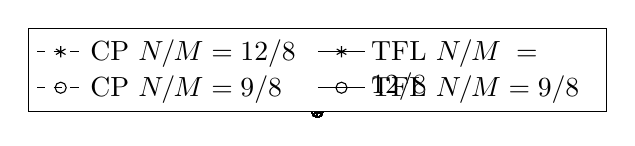
\begin{tikzpicture}

\begin{axis}[%
width=\figurewidth,
height=\figureheight,
at={(0\figurewidth,0\figureheight)},
scale only axis,
separate axis lines,
every outer x axis line/.append style={black},
every x tick label/.append style={font=\color{black}},
xmin=0,
xmax=600,
xlabel={$l_0$},
xmajorgrids,
every outer y axis line/.append style={black},
every y tick label/.append style={font=\color{black}},
ymin=15,
ymax=20,
ylabel={Gain [dB]},
ymajorgrids,
%legend style={legend cell align=left,align=left,draw=black}
legend columns=2,
legend style={text width=8em,legend cell align=left,align=left,draw=black,at={(0.5,1.05)}, anchor=south}
]
\addplot [color=black,dashed,mark=asterisk,mark options={solid}]
  table[row sep=crcr]{%
0	18.2390874094432\\
32	18.2390874094432\\
64	18.2390874094432\\
96	18.2390874094432\\
128	18.2390874094432\\
160	18.2390874094432\\
192	18.2390874094432\\
224	18.2390874094432\\
256	18.2390874094432\\
288	18.2390874094432\\
320	18.2390874094432\\
352	18.2390874094432\\
384	18.2390874094432\\
416	18.2390874094432\\
448	18.2390874094432\\
480	18.2390874094432\\
512	18.2306327719818\\
544	17.9540613758438\\
576	17.6689966399943\\
};
\addlegendentry{CP $N/M=12/8$};

\addplot [color=black,solid,mark=asterisk,mark options={solid}]
  table[row sep=crcr]{%
0	19.9999796047627\\
32	19.9782454264971\\
64	19.9172921503127\\
96	19.819523640774\\
128	19.6869764401989\\
160	19.5221481900787\\
192	19.3264690408576\\
224	19.1028168133025\\
256	18.8524145582619\\
288	18.5769651836831\\
320	18.2797229467138\\
352	17.9588025753321\\
384	17.6198925633198\\
416	17.2597387528296\\
448	16.8807108312221\\
480	16.4832729985219\\
512	16.0669779302672\\
544	15.6289248101717\\
576	15.1692321920288\\
};
\addlegendentry{TFL $N/M=12/8$};

\addplot [color=black,dashed,mark=o,mark options={solid}]
  table[row sep=crcr]{%
0	19.4884747755262\\
32	19.4884747755262\\
64	19.4884747755262\\
96	19.4884747755262\\
128	19.4800794761447\\
160	19.2039363265844\\
192	18.9194155478691\\
224	18.6243664611488\\
256	18.3193439905467\\
288	18.0035198444507\\
320	17.6753775333409\\
352	17.3329477537639\\
384	16.9775142144053\\
416	16.6049465654203\\
448	16.2214034199632\\
480	15.8132879400791\\
512	15.3931020845481\\
544	14.9429381335956\\
576	14.4724841527662\\
};
\addlegendentry{CP $N/M=9/8$};

\addplot [color=black,solid,mark=o,mark options={solid}]
  table[row sep=crcr]{%
0	19.9999188401472\\
32	19.9198402053393\\
64	19.7226565216249\\
96	19.4581952942028\\
128	19.165296513424\\
160	18.8621944283946\\
192	18.5462056497272\\
224	18.2187733804306\\
256	17.8809942229679\\
288	17.5256445475455\\
320	17.1574123511579\\
352	16.769914008492\\
384	16.3698267920046\\
416	15.9497164928657\\
448	15.5024807138218\\
480	15.0375569039195\\
512	14.5394847970002\\
544	14.0174757064722\\
576	13.4597208888491\\
};
\addlegendentry{TFL $N/M=9/8$};

\end{axis}
\end{tikzpicture}%
%  \caption{User interface (internet site/in situ) of the "firefighter team mission"}
%  \label{fig:my-figure}
%\end{figure}

\section{Theory}
\label{sec:theory}

Firstly, a little bit of history for RL : the birth of RL came from the encounter in the late 70s between the computational neurosciences (reinforcement of the synaptic weights of neuronal transmission) and the experimental psychology (animal conditionment models : reinforcement of the behavior leading to satisfaction (ex: Pavlov)) with an adequate mathematical environment : dynamic programming.

A link with experimental psychology is the law of effects of Thorndike (1911) \cite{MUNOS1}
 : "Of several responses made to the same situation, those which are accompanied or closely followed by satisfaction to the animal will, other things being equal, be more firmly connected with the situation, so that, when it recurs, they will be more likely to recur : those which accompanied or closely followed by discomfort to the animal will, other things being equal, have their connections with that situation weakened, so that, when it recurs, they will be less likely to occur. The greater the satisfaction or discomfort, the greater the strenghtening or weakening of the bond".

And so, what is Reinforcement Learning? it is an approach, here computational, to decision-making, understanding and goal-directed learning. The individual learns from direct contact with the environment. It works by the definition of the interactions between a learning agent and its environment in terms of states, actions and rewards. The value and value functions are concepts that are key features of RL methods. Value functions are essential for an efficient search in the space of policies. 

Continuing on that point, what are the objectives of RL?
The objectives of RL are : the automatised acquisition of skills for decision making in a complex and uncertain environment and learning by "experience" a behavioral strategy (named policy) reflecting the failures and success (reinforcements or rewards).

Some examples of achievements of Reinforcement learning are : the production of the best player of backgammon, players of chess, jungling robots, acrobots, etc.

To begin with the theory, we need first to understand what are a Markov chain, a Markov Decision Process (MDP) and dynamic programming \cite{MUNOS1}.

A Markov chain is a dynamic system with discrete time $(x_t)_{t\in\mathbb{N}} \in X$, where $X$ is space of states such as :

\begin{equation*}
\mathbb{P}(x_{t+1}=x|x_t,x_{t-1},...,x_0)=\mathbb{P}(x_{t+1}=x|x_t)
\end{equation*}
giving the Markov property that all the useful information for the future prediction is in the present state. A Markov chain in $X$ is defined by a initial state $x_0$ and the probability of transition $p(y|x)=\mathbb{P}(x_{t+1}=y|x_t=x)$.

Next come the MDP, which is define by $(X,A,p,r)$, where :
\begin{itemize}
 \item $X$ space of states
 \item $A$ space of actions
 \item $p(y|x,a)$ : probability of transition from a state $x \in X$ to $y \in X$ when the action $a \in A$ is chosen:
 \begin{equation*}
 p(y|x,a) = \mathbb{P}(x_{t+1}=y|x_t=x,a_t=a),
 \end{equation*}
 \item $r(x,a,y)$ : reward when passing from $x$ to $y$ using the action $a$.
\end{itemize}
We will note here $V$ the value function and $\pi$ the policy.\\


Dynamic programming possess two types of iterations : iterations on the values and iterations on the policies. Having only interest on the policies, we will develop here only the part concerning the iterations on the policies.
We build a policy sequence, beginning with a given initial policy $\pi_0$, and every step $k$, we evaluate the policy $\pi_k$ and calculate $V^{\pi_k}$, then we improve the policy by calculating $\pi_{k+1}$ given by $V^{\pi_k}$ :
\[ \pi_{k+1}(x) \in \mbox{arg} \mbox{max}_{a \in A}[r(x,a) + \gamma\sum_yp(y|x,a)V^{\pi_k}(y)] 	\]
We stop when $V^{\pi_k} = V^{\pi_{k+1}}$.
It's important to note that the serie $(V^{\pi_k})_k$ is a increasing serie. Therefore, because there is a finite number of possible policies, the termination criteria is obligatory satisfied with k. So we have $V^{\pi_k} = V^*$ where $V^*$ is the optimal value function, therefor $\pi_k$ is the optimal policy.
Some methods of solving are :
\begin{itemize}
 \item \textbf{Direct solving} of the linear system $(I-\gamma P^{\pi})V^{\pi} = r^{\pi}$. That's the Gauss elimination method, but it have a complexity of $O(N^3)$
 \item \textbf{Iteration on the values for a permanent policy} : we iterate on the operator $T^{\pi}$ (Bellman operator). Considering a given value function $V_0$, $V_{n+1} = T^{\pi} V_n$. 
We have then convergence of $V_n$ toward $V^{\pi}$. The problem is that the convergence is asymptotical, but the advantage is that it as a lower complexity that the direct solving method ($O(N^2 \frac{log(1/\epsilon)}{log(1/\gamma)})$ for an approximation of $\epsilon$ (interesting if $\gamma$ is not too close from 1)).
 \item \textbf{Monte-Carlo} : we simulate n trajectories $((x_t^i)_{t \geqslant 0})_{1 \leqslant i \leqslant n}$, starting from $x$ and following the policy $\pi$ : $x_{t+1}^i ~ p(.|x_t^i,\pi(x^i_t))$ , so :
 \begin{equation*}
 V^{\pi}(x) \approx \frac{1}{n} \sum_{i=1}^n \sum_{t \geqslant 0} \gamma^t r(x^i_t, \pi(x^i_t)).
 \end{equation*}
 this method is interesting in we want to evaluate a unique state. It has an approximation error of the order of $O(1/\sqrt{n})$
 \item \textbf{Temporal differences TD($\lambda$)} : This is a smart method for using the trajectories to evaluate all the states crossed by those trajectories, by evaluating the value of a state $x$, by the sum of the observed temporal differences $r_t+\gamma V(x_{t+1}) - V(x_t)$ at the future instants t, ponderate by a "trace" $\lambda$. The algorithm of TD($\lambda$) will be treated later.
\end{itemize}

During the experiments (part Experiments (III)), we used some algorithm (Random method, Cross Enthropy Method (CEM), REINFORCE and TD($\lambda$)). We will focus here on the TD($\lambda$) method, which we found giving the most reliable results during the experiments. It is important to note that the Random method was used to test the functionment of the environment, and the debugging of it.
\\
\textbf{Temporal Differences TD($\lambda$)}
\\
	

\textbf{the algorithm TD($\lambda$)} [Sutton, 1988] : After the observation of a trajectory $(x_0,x_1,...,x_K = 0)$, we update $V_n$	 to the states $(x_k)_0 \leqslant k<K$ following :


\begin{eqnarray*}
V_{n+1}(x_k) = V_n(x_k) + \eta_n(x_k)\sum_{l=k}^{K-1}\lambda^{l-k}d_l,\\ 
\mbox{ where } d_l = r^{\pi}(x_l) + V_n(x_{l+1})-V_n(x_l).
\end{eqnarray*}

%\[ d_l = r^{\pi}(x_l) + V_n(x_{l+1})-V_n(x_l). 	\]


The impact of the temporal differences of future transitions on the estimation of the current state value is updated by $\lambda$. TD($\lambda$) is a compromise between : 
\begin{itemize}
 \item \textbf{TD($0$)} (to estimate the fixed point of the operator of Bellman $T^{\pi}$): 
 \begin{equation*}
  V_{n+1}(x_k) = V_n(x_k) + \eta_n(x_k)d_k. 
 \end{equation*}
 \item \textbf{TD(1)} (to estimate the mean): 
 \begin{equation*} 
 V_{n+1}(x_k) = V_n(x_k) + \eta_n(x_k)\sum_{l>=k}d_l. 
 \end{equation*} 
\end{itemize}

\textbf{implementation of TD($\lambda$)} :

With the eligibility trace $z_n \in \mathbb{R}^N$. Once the transition form $x_k$ to $x_{k+1}$ observated, we can calculate de temporal difference $d_k = r^{\pi}(x_k)+V_n(x_{x+1})-V_n(x_k)$ and update the eligibility trace :


\begin{equation*}
 \left \{
   \begin{split}
    \lambda_{z_{n-1}}(x)  \text{ if } x \ne x_k \\
    1+\lambda_{z_{n-1}}(x) \text{ if } x = x_k \\
    0 \text{ if} x_k = 0
   \end{split}
 \right.
\end{equation*}

and we iterate, for every $x$, 
\begin{equation*}
V_{n+1}(x) = V_n(x) + \eta_n(x)z_n(x)d_n.
\end{equation*}

\textbf{the choice of $\lambda$} :
\begin{itemize}
 \item $\lambda < 1$ allow to reduce the variance of the estemators regarding $\lambda=1$.
 \item $\lambda > 0$ allow to propagate faster the rewards regarding $\lambda=0$.
\end{itemize}

\textbf{the algorithm TD($\lambda$)} in the actualised case :
\begin{equation*}
V_{n+1}(x_k)=V_n(x_k)+\eta_n(x_k)\sum_{t \geqslant k}(\gamma \lambda)^{l-k}d_l.
\end{equation*}

Here was a little introduction to the theory of reinforcement learning and a little zoom on the TD($\lambda$) algorithm that we used during the experimentations of our environment.

\section{Experiment}

We now arrive at the core of this project, which was to develop a learning environment describing the firefighting task in order to improve the policy of the robot and improve its autonomy. For this purpose, we used the toolkit OpenAI Gym, which is a toolkit for developing and comparing reinforcement learning algoriths. We also used the open resource which you can find in the github of torch-twrl (you can follow the link : \url{https://github.com/twitter/torch-twrl}). With this resource, you can run already existing environments such as a cartpole environment, an acrobot, board games, etc.


We used those resources to implement and develop our own environment which was the firefighting task.

The mission that we needed to simulate is a mission of search and fight, here representing a firefighter robot. The mission of the robot is to find trees that are on fire, and extinguish them by spreading water on it.

\textbf{Development of the environment}\\

The first task developed was the most simple one : no moving robot, the only task was to detect if a target was on fire, and then proceed to extinguish it.\\

\begin{figure}
  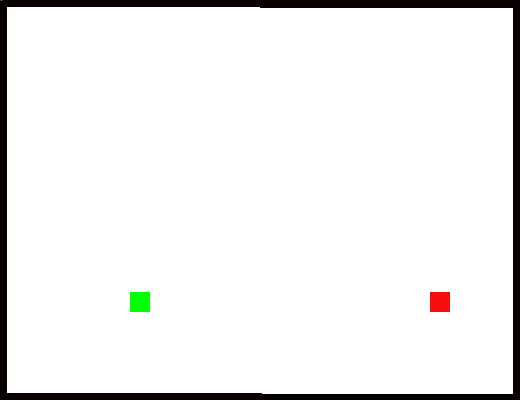
\includegraphics[scale = 0.4]{images/1Dultrasimple.png}
  \caption{View of the simulation of the simple determinist environment}
  \label{fig:my-figure}
\end{figure}

This environment was first developed as determinist. It was an environment where we knew when and where the target will fire up, and see if the robot was able to learn and take measures against.
It's important to note that we used the agent/algorithm cited earlier : TD($\lambda$), REINFORCE, Random agent and CEM.\\

The next step was to turn the determinist environment into a random one, to see if the agents were able to adapt.\\

After studying the adaptability of the agents to the simplest environment possible for our task, the goal was to develop an environment where there was not the only action of extinguishing the target, but also moving to it.\\

\begin{figure}
  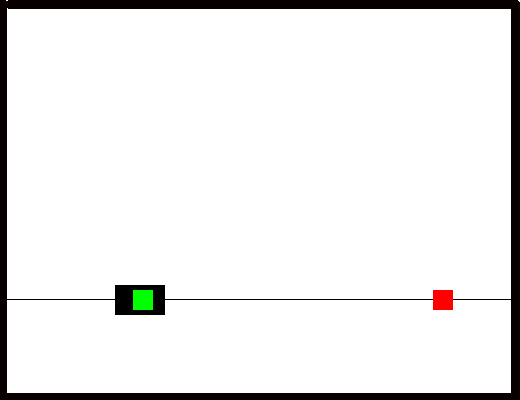
\includegraphics[scale = 0.4]{images/1Dsimple.png}
  \caption{View of the simulation of the 1D environment}
  \label{fig:my-figure}
\end{figure}

The first step was still a determinist environment, where we knew when and where the targets will light up.\\

The second step was to turn the derteminist environment to a random one.

The final step was to develop the 2D environment. The first 2D-environment developed was a simple one, with only targets and the robots. It was used to see if the added actions where working accordingly to the real robot.\\

\begin{figure}
  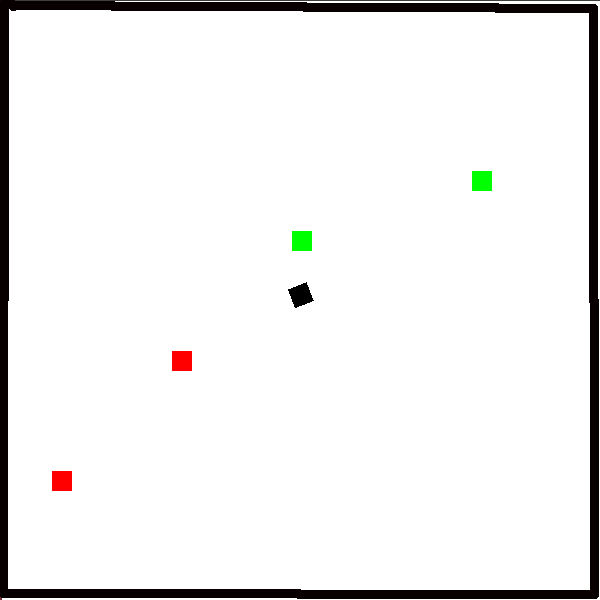
\includegraphics[scale = 0.4]{images/2Dsimple.png}
  \caption{View of the simulation of the 2D environment}
  \label{fig:my-figure}
\end{figure}

Then, we developed a more complex environment to make it as close as possible as reality.\\

\begin{figure}
  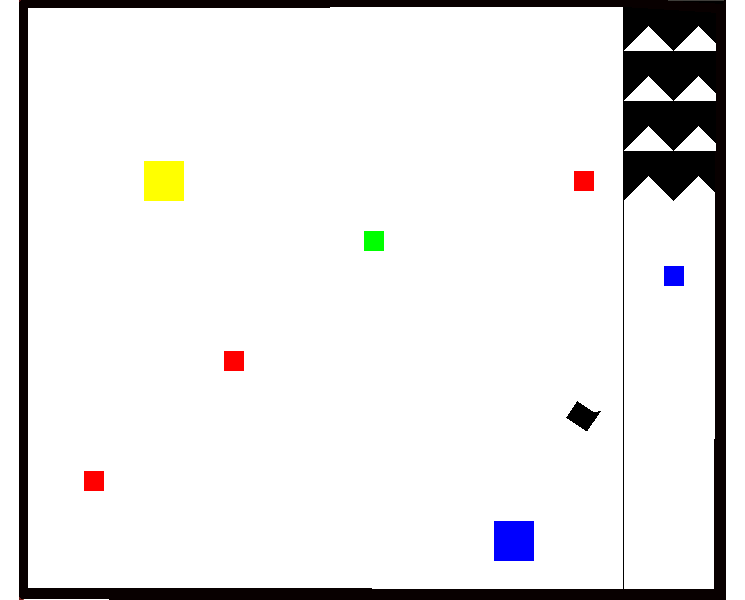
\includegraphics[scale = 0.3]{images/2Dcomplex.png}
  \caption{View of the simulation of the complexified 2D environment}
  \label{fig:my-figure}
\end{figure}

To ensure that the environment was close to reality, we discussed the different drawbacks that we needed to implement :
\begin{itemize}
 \item \textbf{the battery} : the energy available for the robot is not infinite, for this, a decrementing counter was implemented, which was decrementing at every action carried out by the robot. There was also a battery zone where the robot could refill up its energy. The battery zone is modelized by the yellow square.
 \item \textbf{the robot's water reserve} : as for the battery, the water that the robot can carry is not unlimited. The water was implemented as a counter which was decremented every time the agent used the action to spill water. This water could be refilled in the water zone which was represented as a blue square.
 \item \textbf{the refilling water zone} : represented as a blue square, the water refilling zone could see its water level decreasing (which was viewed by the fading blue color) due to water leaks (which are part of the operator actions.). Those leaks
 \item \textbf(the human operator) : the human operator needed to be modelized, as for first, he was designed to not take actions directly on the robot, it was designed to act against the water leaks and fill up the water zone. The operator was designed as a random agent.
 \item \textbf{the temperature} : The temperature needed also to be modelized, as the robot could not stay to long close to a fire. It was modelized as a counter that was increasing when the robot was in a range from the fire, and decreasing when it was out of this range.
 \item \textbf{the fire} : The fires modelized in the environment where fires that could be extinguished with only one application of water. We discussed the fact that we needed more than one action to take care of it, but it was not implemented ultimately. But the idea still lies.
\end{itemize}

\textbf{Experimentation and results}\\

We will focus here on the analysis of the different parameters that we could modify : epsilon, epsilon decate rate, relative alpha and gamma.

You can find the environments and videos of the simulations following this address :
\url{https://github.com/TVagneron/Reinforcement-learning}\\

\textbf{Problems}\\

Some problem occured, and this section is here to describe some of them and maybe help to resolve them.

One of the first issue that we encountered when developping our environment was the definition of the observation space, where we needed to define the observables that can be seen by the agent, as for this we defined the states of the targets by a strict binay duo, 0 when the target was extinguished, 1 if it was lighted. To follow strictly our mathematical model, we used a Tuple to define the target states, but Tuple where not accepted for observation space, so we needed to define them as array and boxes.

The second issue was that when we runned our environment, there was an error ocurring, stating that the local state value was nil. It appears that it was related to a process unable to provide the state at the proper time, resulting in a nil value. This issue was solved by slowing down the process (adding prints to track the error origin solved the proble unexpectedly, but it was also slowed down by adding a wait function in the qfunction). This issue has been observed on two PCs using Ubuntu 14.04. (You can find the issue report following : \url{https://github.com/twitter/torch-twrl/issues/37}).



%\section{First results and future work}

%Equations can be used:
%\begin{equation}
%  \label{eq:tx}
%  s[l] = \sum_{k=0}^{K-1} \sum_{m=0}^{M-1} c_{k,m} g[l-mN] e^{j2\pi \frac{k}{K}l}, \quad l \in \SET{Z}.
%\end{equation}
%Do not forget to define each variable and symbol...

%Figures should be included as floats and properly referenced in the text (Fig. \ref{fig:my-figure}). The same rule applies for tables (Tab. \ref{tab:my-table})

%\begin{figure}[htp]
%  \centering
%  \setlength\figureheight{5cm}
%  \setlength\figurewidth{6cm}
%  % This file was created by matlab2tikz.
% Minimal pgfplots version: 1.3
%
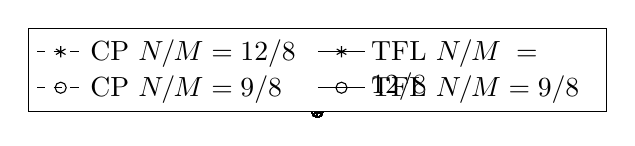
\begin{tikzpicture}

\begin{axis}[%
width=\figurewidth,
height=\figureheight,
at={(0\figurewidth,0\figureheight)},
scale only axis,
separate axis lines,
every outer x axis line/.append style={black},
every x tick label/.append style={font=\color{black}},
xmin=0,
xmax=600,
xlabel={$l_0$},
xmajorgrids,
every outer y axis line/.append style={black},
every y tick label/.append style={font=\color{black}},
ymin=15,
ymax=20,
ylabel={Gain [dB]},
ymajorgrids,
%legend style={legend cell align=left,align=left,draw=black}
legend columns=2,
legend style={text width=8em,legend cell align=left,align=left,draw=black,at={(0.5,1.05)}, anchor=south}
]
\addplot [color=black,dashed,mark=asterisk,mark options={solid}]
  table[row sep=crcr]{%
0	18.2390874094432\\
32	18.2390874094432\\
64	18.2390874094432\\
96	18.2390874094432\\
128	18.2390874094432\\
160	18.2390874094432\\
192	18.2390874094432\\
224	18.2390874094432\\
256	18.2390874094432\\
288	18.2390874094432\\
320	18.2390874094432\\
352	18.2390874094432\\
384	18.2390874094432\\
416	18.2390874094432\\
448	18.2390874094432\\
480	18.2390874094432\\
512	18.2306327719818\\
544	17.9540613758438\\
576	17.6689966399943\\
};
\addlegendentry{CP $N/M=12/8$};

\addplot [color=black,solid,mark=asterisk,mark options={solid}]
  table[row sep=crcr]{%
0	19.9999796047627\\
32	19.9782454264971\\
64	19.9172921503127\\
96	19.819523640774\\
128	19.6869764401989\\
160	19.5221481900787\\
192	19.3264690408576\\
224	19.1028168133025\\
256	18.8524145582619\\
288	18.5769651836831\\
320	18.2797229467138\\
352	17.9588025753321\\
384	17.6198925633198\\
416	17.2597387528296\\
448	16.8807108312221\\
480	16.4832729985219\\
512	16.0669779302672\\
544	15.6289248101717\\
576	15.1692321920288\\
};
\addlegendentry{TFL $N/M=12/8$};

\addplot [color=black,dashed,mark=o,mark options={solid}]
  table[row sep=crcr]{%
0	19.4884747755262\\
32	19.4884747755262\\
64	19.4884747755262\\
96	19.4884747755262\\
128	19.4800794761447\\
160	19.2039363265844\\
192	18.9194155478691\\
224	18.6243664611488\\
256	18.3193439905467\\
288	18.0035198444507\\
320	17.6753775333409\\
352	17.3329477537639\\
384	16.9775142144053\\
416	16.6049465654203\\
448	16.2214034199632\\
480	15.8132879400791\\
512	15.3931020845481\\
544	14.9429381335956\\
576	14.4724841527662\\
};
\addlegendentry{CP $N/M=9/8$};

\addplot [color=black,solid,mark=o,mark options={solid}]
  table[row sep=crcr]{%
0	19.9999188401472\\
32	19.9198402053393\\
64	19.7226565216249\\
96	19.4581952942028\\
128	19.165296513424\\
160	18.8621944283946\\
192	18.5462056497272\\
224	18.2187733804306\\
256	17.8809942229679\\
288	17.5256445475455\\
320	17.1574123511579\\
352	16.769914008492\\
384	16.3698267920046\\
416	15.9497164928657\\
448	15.5024807138218\\
480	15.0375569039195\\
512	14.5394847970002\\
544	14.0174757064722\\
576	13.4597208888491\\
};
\addlegendentry{TFL $N/M=9/8$};

\end{axis}
\end{tikzpicture}%
%  \caption{An accurate caption should be written here}
%  \label{fig:my-figure}
%\end{figure}

%\begin{table}[htp!]
%  \renewcommand{\arraystretch}{1.3}
%  \caption{A detailed caption should be written here}
%  \label{tab:my-table}
%  \centering
%  \begin{tabular}{|c|c|c|c|c|}
%    \hline
%    Filter type & $\sigma_t(\check{\gamma})$ & $\sigma_f(\check{\gamma})$ & $\epsilon_M(\check{\gamma})$ & $\xi(\check{\gamma})$\\
%    \hline
%    RECT & $0.2566N$ & $2.12/M$ & $0.2263$ & $0.1226$\\
%    \hline
%    NR-OBE & $0.2617N$ & $1.44/M$ & $0.1715$ & $0.1874$\\
%    \hline
%    NR-TFL & $0.2580N$ & $0.68/M$ & $0.1839$ & $0.4047$\\
%    \hline
%  \end{tabular}
%\end{table}

% Optional section
%\section*{Acknowledgment}
%The authors would like to thank...



\bibliographystyle{plain}
\bibliography{references}

\end{document}


